\paragraph{Situazione generale} \mbox{}\\
Nella periodo di Verifica e Validazione, a differenza del periodo precedente, l'impegno in ore dei singoli componenti del gruppo è stato omogeneo. Questo perché il numero di ore individuali richieste in questo periodo è di solo 22 ore e anche lo studente lavoratore che ha avuto difficoltà in precedenza è riuscito a soddisfarle tutte.\\
In seguito all'incontro con la Proponente è stato necessario valutare l'implementazione di alcune proposte fatte per l'applicativo finale. Per questo motivo a fine periodo si rileva uno scostamento di 3 ore dal ruolo di \progr{} al ruolo di \textit{Progettista} rispetto a quanto preventivato in precedenza. Questo cambiamento non ha influenzato il numero di ore individuali, ma ha aumentato il costo finale di 21,00\euro. \\
In questo periodo non sono state riscontrate particolari difficoltà, tranne per le differenze nell'orario di lavoro dei membri che sono state in parte risolte incontrandosi soprattutto nei week-end. L'armonia all'interno del gruppo è rimasta buona.\\

\begin{figure}[H]
	\centering
	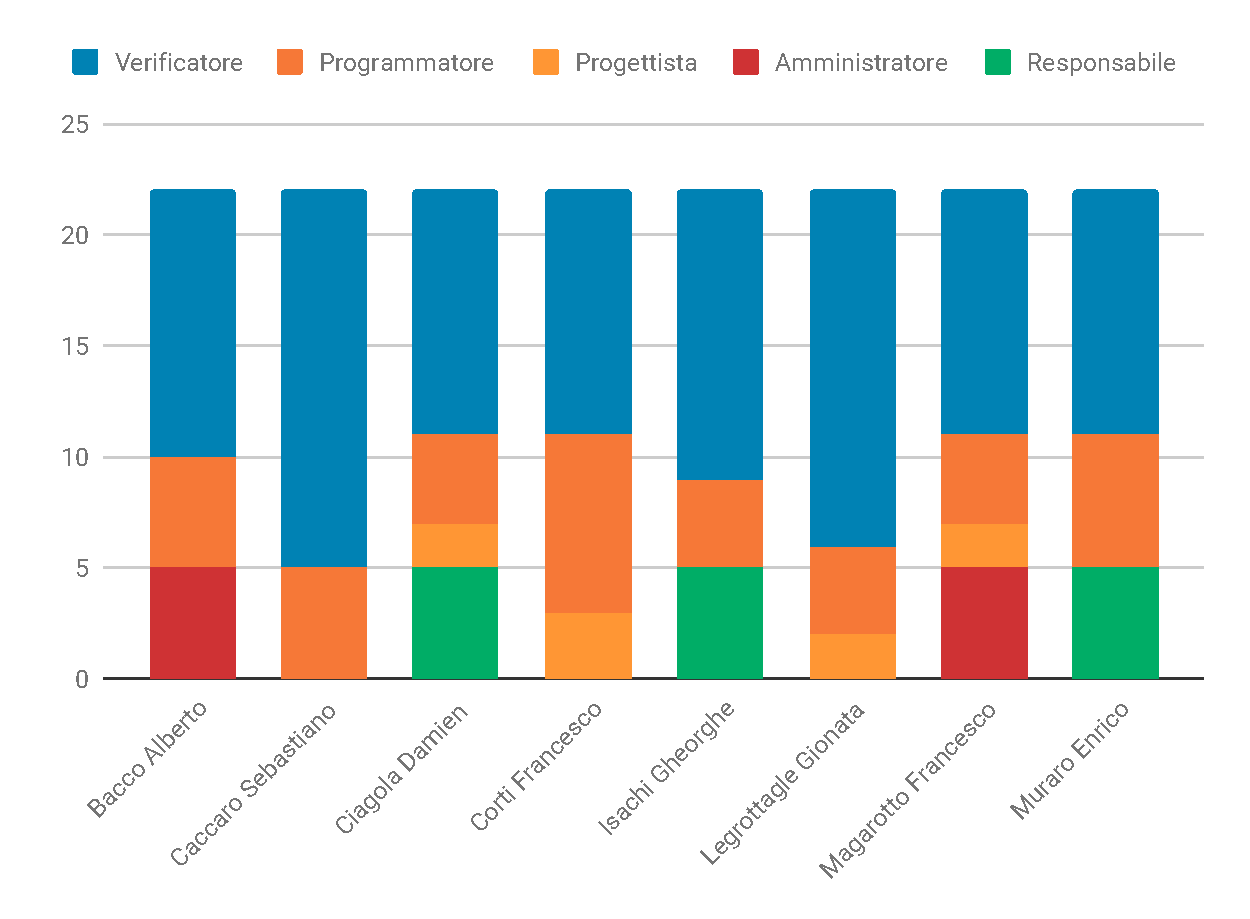
\includegraphics[scale=.8]{Consuntivo/grafici/ConsVer.pdf} 
	\caption{Grafico orario per componente a fine periodo}
\end{figure}